\section*{Výsledky měření}
Použili jsme síťové napětí ($f \approx \SI{0.02}{\radian\per\second}$).

Nejdříve jsme změřili účiníky rezistoru, kondenzátoru ($C=\SI{10}{\micro\farad}$) a cívky pomocí analogového a digitálního wattmetru.
Při měření analogovým wattmetrem jsme napětí měřili multimetrem MXD 4660A a proud multimetrem MASTECH MY 65, chybu jsme odhadli s ohledem na oscilaci číslic na displeji.
Výsledky jsou shrnuty v tabulce \ref{t:jednicka}.
Digitální wattmetr umožňoval odečítat přímo účiník, takže ve sloupci $\cos\varphi$ budu uvádět účiník vypočtený z \eqref{e:ucinik} a ve sloupci PF účiník odečtený wattmetrem.
Chybu veličin měřených digitálních voltmetrem považujeme za řád poslední číslice na displeji, dále neuvádíme.
Chybu anologového wattmetru jsme odhadli podle nejmenšího dílku stupnice, který byl \SI{25}{\milli\watt}.
Chyby nepřímo měřených veličin počítáme metodou přenosu chyb, přičemž chybu fázového posuvu $\varphi$ navíc odhadujeme s ohledem na přesnost metody.


\begin{tabulka}[htbp]
\centering
\begin{tabular}{c|c|cccccc}
wattmetr & součástka & $U$ (\si{\volt}) & $I$ (\si{\milli\ampere}) & $P$ (\si{\watt}) & $\cos \varphi$ & PF & $\varphi$ (\si{\degree}) \\ \hline
\multirow{3}{*}{analogový} & R & \num{53.6(1)} & \num{53.8(2)} & \num{2.8(1)} & \num{0.97(4)} & --- & \num{0(13)} \\
 & C & \num{57.20(5)} & \num{178.0(5)} & \num{0.0(1)} & \num{0.00(1)} & --- &\num{-90(1)} \\
 & L & \num{56.0(1)} & \num{31.90(5)} & \num{0.63(1)} & \num{0.35(6)} & --- &\num{70(1)} \\ \hline
\multirow{3}{*}{digitální} & R & \num{51.6(1)} & \num{52(1)} & \num{2.695(1)} & \num{1.00(2)} & \num{1.00} &\num{0(5)} \\
 & C & \num{53.7(1)} & \num{172(1)} & \num{0.016(1)} & \num{0.002(1)} & \num{0.00} &\num{-89.9(1)} \\
 & L & \num{52.5(1)} & \num{30(1)} & \num{0.645(1)} & \num{0.41(2)} & \num{0.40} &\num{65.8(2)} \\
\end{tabular}
\caption{Účiník rezistoru, kondenzátoru a cívky}
\label{t:jednicka}
\end{tabulka}

Podle \eqref{e:ser} a \eqref{e:par} jsme určili sériové
\begin{equation*}
R_S=\SI{720(50)}{\ohm} \qquad \qquad L_S=\SI{5.1(2)}{\henry}
\end{equation*}
a paralelní
\begin{equation*}
R_P=\SI{4270(50)}{\ohm} \qquad \qquad L_P=\SI{6.1(2)}{\henry}
\end{equation*}
náhradní zapojení cívky. K výpočtu jsme použili hodnoty z digitálního wattmetru, protože jsou přesnější.

Změřili jsme účiník seriového a paralelního RC obvodu.
Výsledky jsou shrnuty v tabulce \ref{t:RC} a grafech \ref{g:RCucinik} a \ref{g:RCfaze}.
Chybu kapacitní dekády odhadujeme na \SI{1}{\percent}.
Chybu ostatních veličin považujeme za řád poslední uvedené číslice.
Chybu odporu jsme počítali metodou přenosu chyb ze vzorců \eqref{e:RCs} a \eqref{e:RCp}.

\begin{tabulka}[htbp]
\centering
\begin{tabular}{ccccccc|c}
\multicolumn{8}{c}{sériový RC obvod} \\
$C$ (\si{\micro\farad}) & $U$ (\si{\volt}) & $I$ (\si{\milli\ampere}) & $P$ (\si{\watt}) & $\cos \varphi$ & PF & $\varphi$ (\si{\degree}) &  $R_s$ (\si{\ohm})    \\ \hline
\num{1} & \num{52.8} & \num{15} & \num{0.30} & \num{0.38} & --- & \num{-67} & \num{1330(200)} \\
\num{2} & \num{52.8} & \num{28} & \num{0.80} & \num{0.54} & \num{0.53} & \num{-57} & \num{1020(80)} \\
\num{5} & \num{52.2} & \num{44} & \num{1.95} & \num{0.85} & \num{0.84} & \num{-32} & \num{1010(50)} \\
\num{10} & \num{51.7} & \num{50} & \num{2.47} & \num{0.95} & \num{0.95} & \num{-17} & \num{990(40)} \\
\hline \hline
\multicolumn{8}{c}{paralelní RC obvod} \\
$C$ (\si{\micro\farad}) & $U$ (\si{\volt}) & $I$ (\si{\milli\ampere}) & $P$ (\si{\watt}) & $\cos \varphi$ & PF & $\varphi$ (\si{\degree}) & $R_p$ (\si{\ohm}) \\ \hline
\num{1} & \num{51.8} & \num{55} & \num{2.70} & \num{0.95} & \num{0.96} & \num{-19} & \num{994(6)} \\
\num{2} & \num{51.8} & \num{62} & \num{2.71} & \num{0.84} & \num{0.84} & \num{-32} & \num{990(6)} \\
\num{5} & \num{52.0} & \num{99} & \num{2.73} & \num{0.53} & \num{0.53} & \num{-58} & \num{990(6)} \\
\num{10} & \num{52.4} & \num{174} & \num{2.79} & \num{0.31} & \num{0.31} & \num{-72} & \num{984(6)} \\

\end{tabular}
\caption{Účiník RC obvodu}
\label{t:RC}
\end{tabulka}

\begin{graph}[htbp] 
\centering
% GNUPLOT: LaTeX picture with Postscript
\begingroup
  \makeatletter
  \providecommand\color[2][]{%
    \GenericError{(gnuplot) \space\space\space\@spaces}{%
      Package color not loaded in conjunction with
      terminal option `colourtext'%
    }{See the gnuplot documentation for explanation.%
    }{Either use 'blacktext' in gnuplot or load the package
      color.sty in LaTeX.}%
    \renewcommand\color[2][]{}%
  }%
  \providecommand\includegraphics[2][]{%
    \GenericError{(gnuplot) \space\space\space\@spaces}{%
      Package graphicx or graphics not loaded%
    }{See the gnuplot documentation for explanation.%
    }{The gnuplot epslatex terminal needs graphicx.sty or graphics.sty.}%
    \renewcommand\includegraphics[2][]{}%
  }%
  \providecommand\rotatebox[2]{#2}%
  \@ifundefined{ifGPcolor}{%
    \newif\ifGPcolor
    \GPcolorfalse
  }{}%
  \@ifundefined{ifGPblacktext}{%
    \newif\ifGPblacktext
    \GPblacktexttrue
  }{}%
  % define a \g@addto@macro without @ in the name:
  \let\gplgaddtomacro\g@addto@macro
  % define empty templates for all commands taking text:
  \gdef\gplbacktext{}%
  \gdef\gplfronttext{}%
  \makeatother
  \ifGPblacktext
    % no textcolor at all
    \def\colorrgb#1{}%
    \def\colorgray#1{}%
  \else
    % gray or color?
    \ifGPcolor
      \def\colorrgb#1{\color[rgb]{#1}}%
      \def\colorgray#1{\color[gray]{#1}}%
      \expandafter\def\csname LTw\endcsname{\color{white}}%
      \expandafter\def\csname LTb\endcsname{\color{black}}%
      \expandafter\def\csname LTa\endcsname{\color{black}}%
      \expandafter\def\csname LT0\endcsname{\color[rgb]{1,0,0}}%
      \expandafter\def\csname LT1\endcsname{\color[rgb]{0,1,0}}%
      \expandafter\def\csname LT2\endcsname{\color[rgb]{0,0,1}}%
      \expandafter\def\csname LT3\endcsname{\color[rgb]{1,0,1}}%
      \expandafter\def\csname LT4\endcsname{\color[rgb]{0,1,1}}%
      \expandafter\def\csname LT5\endcsname{\color[rgb]{1,1,0}}%
      \expandafter\def\csname LT6\endcsname{\color[rgb]{0,0,0}}%
      \expandafter\def\csname LT7\endcsname{\color[rgb]{1,0.3,0}}%
      \expandafter\def\csname LT8\endcsname{\color[rgb]{0.5,0.5,0.5}}%
    \else
      % gray
      \def\colorrgb#1{\color{black}}%
      \def\colorgray#1{\color[gray]{#1}}%
      \expandafter\def\csname LTw\endcsname{\color{white}}%
      \expandafter\def\csname LTb\endcsname{\color{black}}%
      \expandafter\def\csname LTa\endcsname{\color{black}}%
      \expandafter\def\csname LT0\endcsname{\color{black}}%
      \expandafter\def\csname LT1\endcsname{\color{black}}%
      \expandafter\def\csname LT2\endcsname{\color{black}}%
      \expandafter\def\csname LT3\endcsname{\color{black}}%
      \expandafter\def\csname LT4\endcsname{\color{black}}%
      \expandafter\def\csname LT5\endcsname{\color{black}}%
      \expandafter\def\csname LT6\endcsname{\color{black}}%
      \expandafter\def\csname LT7\endcsname{\color{black}}%
      \expandafter\def\csname LT8\endcsname{\color{black}}%
    \fi
  \fi
  \setlength{\unitlength}{0.0500bp}%
  \begin{picture}(7936.00,5668.00)%
    \gplgaddtomacro\gplbacktext{%
      \csname LTb\endcsname%
      \put(946,704){\makebox(0,0)[r]{\strut{} 0}}%
      \csname LTb\endcsname%
      \put(946,1644){\makebox(0,0)[r]{\strut{} 0.2}}%
      \csname LTb\endcsname%
      \put(946,2584){\makebox(0,0)[r]{\strut{} 0.4}}%
      \csname LTb\endcsname%
      \put(946,3523){\makebox(0,0)[r]{\strut{} 0.6}}%
      \csname LTb\endcsname%
      \put(946,4463){\makebox(0,0)[r]{\strut{} 0.8}}%
      \csname LTb\endcsname%
      \put(946,5403){\makebox(0,0)[r]{\strut{} 1}}%
      \csname LTb\endcsname%
      \put(1078,484){\makebox(0,0){\strut{} 0}}%
      \csname LTb\endcsname%
      \put(2253,484){\makebox(0,0){\strut{} 2}}%
      \csname LTb\endcsname%
      \put(3427,484){\makebox(0,0){\strut{} 4}}%
      \csname LTb\endcsname%
      \put(4602,484){\makebox(0,0){\strut{} 6}}%
      \csname LTb\endcsname%
      \put(5777,484){\makebox(0,0){\strut{} 8}}%
      \csname LTb\endcsname%
      \put(6952,484){\makebox(0,0){\strut{} 10}}%
      \put(176,3053){\rotatebox{-270}{\makebox(0,0){\strut{}$\cos\varphi$}}}%
      \put(4308,154){\makebox(0,0){\strut{}$C$ (\si{\micro\farad})}}%
    }%
    \gplgaddtomacro\gplfronttext{%
      \csname LTb\endcsname%
      \put(2530,1097){\makebox(0,0)[r]{\strut{}sériový}}%
      \csname LTb\endcsname%
      \put(2530,877){\makebox(0,0)[r]{\strut{}paralelní}}%
    }%
    \gplbacktext
    \put(0,0){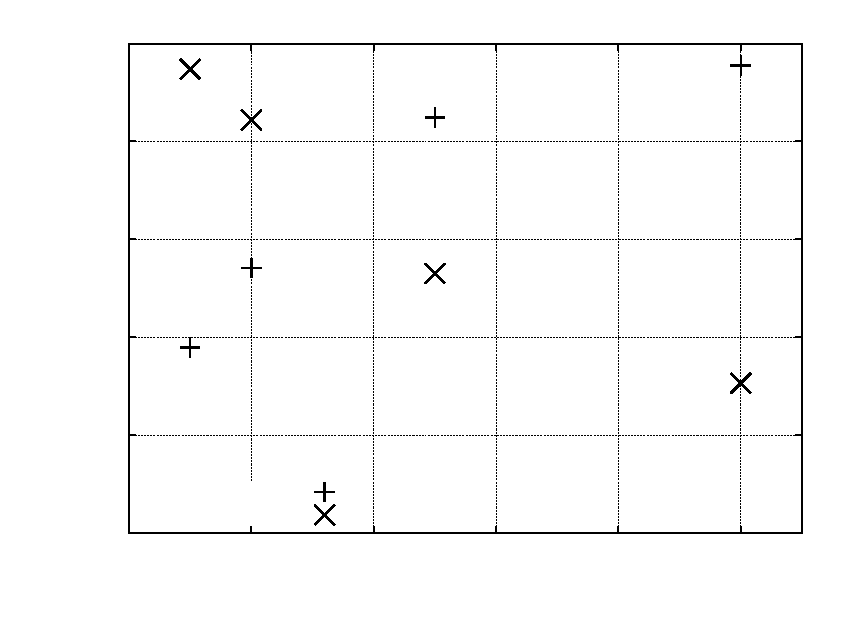
\includegraphics{RCu}}%
    \gplfronttext
  \end{picture}%
\endgroup

\caption{Účiník RC obvodu v závislosti na $C$}
\label{g:RCucinik}
\end{graph}

\begin{graph}[htbp] 
\centering
% GNUPLOT: LaTeX picture with Postscript
\begingroup
  \makeatletter
  \providecommand\color[2][]{%
    \GenericError{(gnuplot) \space\space\space\@spaces}{%
      Package color not loaded in conjunction with
      terminal option `colourtext'%
    }{See the gnuplot documentation for explanation.%
    }{Either use 'blacktext' in gnuplot or load the package
      color.sty in LaTeX.}%
    \renewcommand\color[2][]{}%
  }%
  \providecommand\includegraphics[2][]{%
    \GenericError{(gnuplot) \space\space\space\@spaces}{%
      Package graphicx or graphics not loaded%
    }{See the gnuplot documentation for explanation.%
    }{The gnuplot epslatex terminal needs graphicx.sty or graphics.sty.}%
    \renewcommand\includegraphics[2][]{}%
  }%
  \providecommand\rotatebox[2]{#2}%
  \@ifundefined{ifGPcolor}{%
    \newif\ifGPcolor
    \GPcolorfalse
  }{}%
  \@ifundefined{ifGPblacktext}{%
    \newif\ifGPblacktext
    \GPblacktexttrue
  }{}%
  % define a \g@addto@macro without @ in the name:
  \let\gplgaddtomacro\g@addto@macro
  % define empty templates for all commands taking text:
  \gdef\gplbacktext{}%
  \gdef\gplfronttext{}%
  \makeatother
  \ifGPblacktext
    % no textcolor at all
    \def\colorrgb#1{}%
    \def\colorgray#1{}%
  \else
    % gray or color?
    \ifGPcolor
      \def\colorrgb#1{\color[rgb]{#1}}%
      \def\colorgray#1{\color[gray]{#1}}%
      \expandafter\def\csname LTw\endcsname{\color{white}}%
      \expandafter\def\csname LTb\endcsname{\color{black}}%
      \expandafter\def\csname LTa\endcsname{\color{black}}%
      \expandafter\def\csname LT0\endcsname{\color[rgb]{1,0,0}}%
      \expandafter\def\csname LT1\endcsname{\color[rgb]{0,1,0}}%
      \expandafter\def\csname LT2\endcsname{\color[rgb]{0,0,1}}%
      \expandafter\def\csname LT3\endcsname{\color[rgb]{1,0,1}}%
      \expandafter\def\csname LT4\endcsname{\color[rgb]{0,1,1}}%
      \expandafter\def\csname LT5\endcsname{\color[rgb]{1,1,0}}%
      \expandafter\def\csname LT6\endcsname{\color[rgb]{0,0,0}}%
      \expandafter\def\csname LT7\endcsname{\color[rgb]{1,0.3,0}}%
      \expandafter\def\csname LT8\endcsname{\color[rgb]{0.5,0.5,0.5}}%
    \else
      % gray
      \def\colorrgb#1{\color{black}}%
      \def\colorgray#1{\color[gray]{#1}}%
      \expandafter\def\csname LTw\endcsname{\color{white}}%
      \expandafter\def\csname LTb\endcsname{\color{black}}%
      \expandafter\def\csname LTa\endcsname{\color{black}}%
      \expandafter\def\csname LT0\endcsname{\color{black}}%
      \expandafter\def\csname LT1\endcsname{\color{black}}%
      \expandafter\def\csname LT2\endcsname{\color{black}}%
      \expandafter\def\csname LT3\endcsname{\color{black}}%
      \expandafter\def\csname LT4\endcsname{\color{black}}%
      \expandafter\def\csname LT5\endcsname{\color{black}}%
      \expandafter\def\csname LT6\endcsname{\color{black}}%
      \expandafter\def\csname LT7\endcsname{\color{black}}%
      \expandafter\def\csname LT8\endcsname{\color{black}}%
    \fi
  \fi
  \setlength{\unitlength}{0.0500bp}%
  \begin{picture}(7936.00,5668.00)%
    \gplgaddtomacro\gplbacktext{%
      \csname LTb\endcsname%
      \put(814,704){\makebox(0,0)[r]{\strut{}-90}}%
      \csname LTb\endcsname%
      \put(814,1226){\makebox(0,0)[r]{\strut{}-80}}%
      \csname LTb\endcsname%
      \put(814,1748){\makebox(0,0)[r]{\strut{}-70}}%
      \csname LTb\endcsname%
      \put(814,2270){\makebox(0,0)[r]{\strut{}-60}}%
      \csname LTb\endcsname%
      \put(814,2792){\makebox(0,0)[r]{\strut{}-50}}%
      \csname LTb\endcsname%
      \put(814,3315){\makebox(0,0)[r]{\strut{}-40}}%
      \csname LTb\endcsname%
      \put(814,3837){\makebox(0,0)[r]{\strut{}-30}}%
      \csname LTb\endcsname%
      \put(814,4359){\makebox(0,0)[r]{\strut{}-20}}%
      \csname LTb\endcsname%
      \put(814,4881){\makebox(0,0)[r]{\strut{}-10}}%
      \csname LTb\endcsname%
      \put(814,5403){\makebox(0,0)[r]{\strut{} 0}}%
      \csname LTb\endcsname%
      \put(946,484){\makebox(0,0){\strut{} 0}}%
      \csname LTb\endcsname%
      \put(2145,484){\makebox(0,0){\strut{} 2}}%
      \csname LTb\endcsname%
      \put(3343,484){\makebox(0,0){\strut{} 4}}%
      \csname LTb\endcsname%
      \put(4542,484){\makebox(0,0){\strut{} 6}}%
      \csname LTb\endcsname%
      \put(5741,484){\makebox(0,0){\strut{} 8}}%
      \csname LTb\endcsname%
      \put(6940,484){\makebox(0,0){\strut{} 10}}%
      \put(176,3053){\rotatebox{-270}{\makebox(0,0){\strut{}$\varphi$ (\si{\degree})}}}%
      \put(4242,154){\makebox(0,0){\strut{}$C$ (\si{\micro\farad})}}%
    }%
    \gplgaddtomacro\gplfronttext{%
      \csname LTb\endcsname%
      \put(2398,1097){\makebox(0,0)[r]{\strut{}sériový}}%
      \csname LTb\endcsname%
      \put(2398,877){\makebox(0,0)[r]{\strut{}paralelní}}%
    }%
    \gplbacktext
    \put(0,0){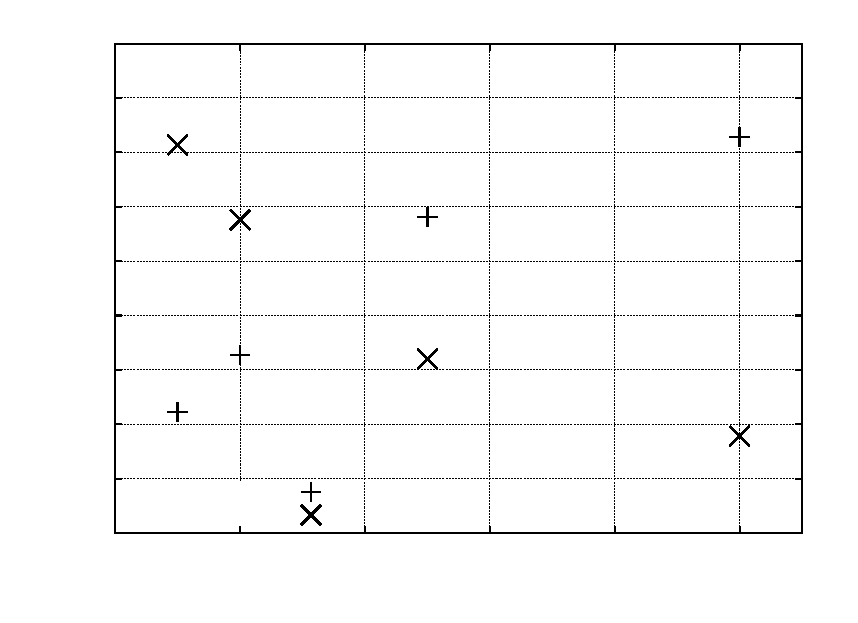
\includegraphics{RCf}}%
    \gplfronttext
  \end{picture}%
\endgroup

\caption{Fázové posunutí proudu vůči napětí v RC obvodu v závislosti na $C$}
\label{g:RCfaze}
\end{graph}

S přihlédnutím k jednotlivým hodnotám $R$ v tabulce \ref{t:RC} a jejich odchylkám můžeme usoudit, že správná hodnota je $R=\SI{990(5)}{\ohm}$.
Odpor jsme změřili i digitálním multimetrem MXD 4660A, jeho hodnota byla \SI{982(2)}{\kilo\ohm}.

Dále jsme změřili závislost proudu a výkonu na velikosti kapacity zařazené do sériového RLC obvodu.
Výsledky jsou shrnuty v tabulce na přiloženém papíře a v grafech \ref{g:RLCu}, \ref{g:RLCf} a \ref{g:RLCP}.
Při výpočtu $\varphi$ jsme použili hodnoty ze sloupečku $\cos\varphi$, ne PF.

\begin{graph}[htbp] 
\centering
% GNUPLOT: LaTeX picture with Postscript
\begingroup
  \makeatletter
  \providecommand\color[2][]{%
    \GenericError{(gnuplot) \space\space\space\@spaces}{%
      Package color not loaded in conjunction with
      terminal option `colourtext'%
    }{See the gnuplot documentation for explanation.%
    }{Either use 'blacktext' in gnuplot or load the package
      color.sty in LaTeX.}%
    \renewcommand\color[2][]{}%
  }%
  \providecommand\includegraphics[2][]{%
    \GenericError{(gnuplot) \space\space\space\@spaces}{%
      Package graphicx or graphics not loaded%
    }{See the gnuplot documentation for explanation.%
    }{The gnuplot epslatex terminal needs graphicx.sty or graphics.sty.}%
    \renewcommand\includegraphics[2][]{}%
  }%
  \providecommand\rotatebox[2]{#2}%
  \@ifundefined{ifGPcolor}{%
    \newif\ifGPcolor
    \GPcolorfalse
  }{}%
  \@ifundefined{ifGPblacktext}{%
    \newif\ifGPblacktext
    \GPblacktexttrue
  }{}%
  % define a \g@addto@macro without @ in the name:
  \let\gplgaddtomacro\g@addto@macro
  % define empty templates for all commands taking text:
  \gdef\gplbacktext{}%
  \gdef\gplfronttext{}%
  \makeatother
  \ifGPblacktext
    % no textcolor at all
    \def\colorrgb#1{}%
    \def\colorgray#1{}%
  \else
    % gray or color?
    \ifGPcolor
      \def\colorrgb#1{\color[rgb]{#1}}%
      \def\colorgray#1{\color[gray]{#1}}%
      \expandafter\def\csname LTw\endcsname{\color{white}}%
      \expandafter\def\csname LTb\endcsname{\color{black}}%
      \expandafter\def\csname LTa\endcsname{\color{black}}%
      \expandafter\def\csname LT0\endcsname{\color[rgb]{1,0,0}}%
      \expandafter\def\csname LT1\endcsname{\color[rgb]{0,1,0}}%
      \expandafter\def\csname LT2\endcsname{\color[rgb]{0,0,1}}%
      \expandafter\def\csname LT3\endcsname{\color[rgb]{1,0,1}}%
      \expandafter\def\csname LT4\endcsname{\color[rgb]{0,1,1}}%
      \expandafter\def\csname LT5\endcsname{\color[rgb]{1,1,0}}%
      \expandafter\def\csname LT6\endcsname{\color[rgb]{0,0,0}}%
      \expandafter\def\csname LT7\endcsname{\color[rgb]{1,0.3,0}}%
      \expandafter\def\csname LT8\endcsname{\color[rgb]{0.5,0.5,0.5}}%
    \else
      % gray
      \def\colorrgb#1{\color{black}}%
      \def\colorgray#1{\color[gray]{#1}}%
      \expandafter\def\csname LTw\endcsname{\color{white}}%
      \expandafter\def\csname LTb\endcsname{\color{black}}%
      \expandafter\def\csname LTa\endcsname{\color{black}}%
      \expandafter\def\csname LT0\endcsname{\color{black}}%
      \expandafter\def\csname LT1\endcsname{\color{black}}%
      \expandafter\def\csname LT2\endcsname{\color{black}}%
      \expandafter\def\csname LT3\endcsname{\color{black}}%
      \expandafter\def\csname LT4\endcsname{\color{black}}%
      \expandafter\def\csname LT5\endcsname{\color{black}}%
      \expandafter\def\csname LT6\endcsname{\color{black}}%
      \expandafter\def\csname LT7\endcsname{\color{black}}%
      \expandafter\def\csname LT8\endcsname{\color{black}}%
    \fi
  \fi
  \setlength{\unitlength}{0.0500bp}%
  \begin{picture}(7936.00,5668.00)%
    \gplgaddtomacro\gplbacktext{%
      \csname LTb\endcsname%
      \put(946,704){\makebox(0,0)[r]{\strut{} 0}}%
      \csname LTb\endcsname%
      \put(946,1558){\makebox(0,0)[r]{\strut{} 0.2}}%
      \csname LTb\endcsname%
      \put(946,2413){\makebox(0,0)[r]{\strut{} 0.4}}%
      \csname LTb\endcsname%
      \put(946,3267){\makebox(0,0)[r]{\strut{} 0.6}}%
      \csname LTb\endcsname%
      \put(946,4121){\makebox(0,0)[r]{\strut{} 0.8}}%
      \csname LTb\endcsname%
      \put(946,4976){\makebox(0,0)[r]{\strut{} 1}}%
      \csname LTb\endcsname%
      \put(1078,484){\makebox(0,0){\strut{} 0}}%
      \csname LTb\endcsname%
      \put(2253,484){\makebox(0,0){\strut{} 2}}%
      \csname LTb\endcsname%
      \put(3427,484){\makebox(0,0){\strut{} 4}}%
      \csname LTb\endcsname%
      \put(4602,484){\makebox(0,0){\strut{} 6}}%
      \csname LTb\endcsname%
      \put(5777,484){\makebox(0,0){\strut{} 8}}%
      \csname LTb\endcsname%
      \put(6952,484){\makebox(0,0){\strut{} 10}}%
      \put(176,3053){\rotatebox{-270}{\makebox(0,0){\strut{}$\cos\varphi$}}}%
      \put(4308,154){\makebox(0,0){\strut{}$C$ (\si{\micro\farad})}}%
    }%
    \gplgaddtomacro\gplfronttext{%
    }%
    \gplbacktext
    \put(0,0){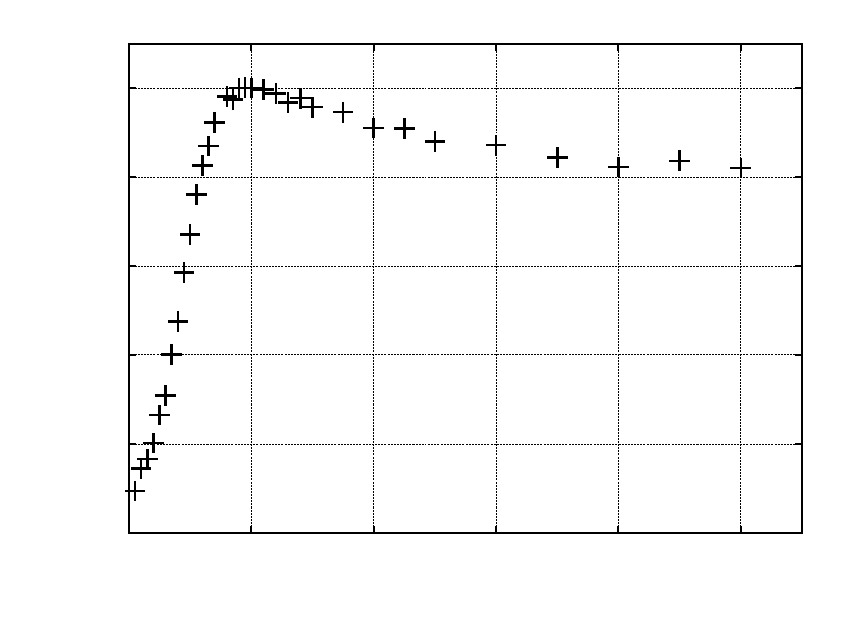
\includegraphics{RLCu}}%
    \gplfronttext
  \end{picture}%
\endgroup

\caption{Účiník RLC obvodu v závislosti na $C$}
\label{g:RLCu}
\end{graph}

\begin{graph}[htbp] 
\centering
% GNUPLOT: LaTeX picture with Postscript
\begingroup
  \makeatletter
  \providecommand\color[2][]{%
    \GenericError{(gnuplot) \space\space\space\@spaces}{%
      Package color not loaded in conjunction with
      terminal option `colourtext'%
    }{See the gnuplot documentation for explanation.%
    }{Either use 'blacktext' in gnuplot or load the package
      color.sty in LaTeX.}%
    \renewcommand\color[2][]{}%
  }%
  \providecommand\includegraphics[2][]{%
    \GenericError{(gnuplot) \space\space\space\@spaces}{%
      Package graphicx or graphics not loaded%
    }{See the gnuplot documentation for explanation.%
    }{The gnuplot epslatex terminal needs graphicx.sty or graphics.sty.}%
    \renewcommand\includegraphics[2][]{}%
  }%
  \providecommand\rotatebox[2]{#2}%
  \@ifundefined{ifGPcolor}{%
    \newif\ifGPcolor
    \GPcolorfalse
  }{}%
  \@ifundefined{ifGPblacktext}{%
    \newif\ifGPblacktext
    \GPblacktexttrue
  }{}%
  % define a \g@addto@macro without @ in the name:
  \let\gplgaddtomacro\g@addto@macro
  % define empty templates for all commands taking text:
  \gdef\gplbacktext{}%
  \gdef\gplfronttext{}%
  \makeatother
  \ifGPblacktext
    % no textcolor at all
    \def\colorrgb#1{}%
    \def\colorgray#1{}%
  \else
    % gray or color?
    \ifGPcolor
      \def\colorrgb#1{\color[rgb]{#1}}%
      \def\colorgray#1{\color[gray]{#1}}%
      \expandafter\def\csname LTw\endcsname{\color{white}}%
      \expandafter\def\csname LTb\endcsname{\color{black}}%
      \expandafter\def\csname LTa\endcsname{\color{black}}%
      \expandafter\def\csname LT0\endcsname{\color[rgb]{1,0,0}}%
      \expandafter\def\csname LT1\endcsname{\color[rgb]{0,1,0}}%
      \expandafter\def\csname LT2\endcsname{\color[rgb]{0,0,1}}%
      \expandafter\def\csname LT3\endcsname{\color[rgb]{1,0,1}}%
      \expandafter\def\csname LT4\endcsname{\color[rgb]{0,1,1}}%
      \expandafter\def\csname LT5\endcsname{\color[rgb]{1,1,0}}%
      \expandafter\def\csname LT6\endcsname{\color[rgb]{0,0,0}}%
      \expandafter\def\csname LT7\endcsname{\color[rgb]{1,0.3,0}}%
      \expandafter\def\csname LT8\endcsname{\color[rgb]{0.5,0.5,0.5}}%
    \else
      % gray
      \def\colorrgb#1{\color{black}}%
      \def\colorgray#1{\color[gray]{#1}}%
      \expandafter\def\csname LTw\endcsname{\color{white}}%
      \expandafter\def\csname LTb\endcsname{\color{black}}%
      \expandafter\def\csname LTa\endcsname{\color{black}}%
      \expandafter\def\csname LT0\endcsname{\color{black}}%
      \expandafter\def\csname LT1\endcsname{\color{black}}%
      \expandafter\def\csname LT2\endcsname{\color{black}}%
      \expandafter\def\csname LT3\endcsname{\color{black}}%
      \expandafter\def\csname LT4\endcsname{\color{black}}%
      \expandafter\def\csname LT5\endcsname{\color{black}}%
      \expandafter\def\csname LT6\endcsname{\color{black}}%
      \expandafter\def\csname LT7\endcsname{\color{black}}%
      \expandafter\def\csname LT8\endcsname{\color{black}}%
    \fi
  \fi
  \setlength{\unitlength}{0.0500bp}%
  \begin{picture}(7936.00,5668.00)%
    \gplgaddtomacro\gplbacktext{%
      \csname LTb\endcsname%
      \put(814,704){\makebox(0,0)[r]{\strut{}-90}}%
      \csname LTb\endcsname%
      \put(814,1487){\makebox(0,0)[r]{\strut{}-60}}%
      \csname LTb\endcsname%
      \put(814,2270){\makebox(0,0)[r]{\strut{}-30}}%
      \csname LTb\endcsname%
      \put(814,3054){\makebox(0,0)[r]{\strut{} 0}}%
      \csname LTb\endcsname%
      \put(814,3837){\makebox(0,0)[r]{\strut{} 30}}%
      \csname LTb\endcsname%
      \put(814,4620){\makebox(0,0)[r]{\strut{} 60}}%
      \csname LTb\endcsname%
      \put(814,5403){\makebox(0,0)[r]{\strut{} 90}}%
      \csname LTb\endcsname%
      \put(946,484){\makebox(0,0){\strut{} 0}}%
      \csname LTb\endcsname%
      \put(2145,484){\makebox(0,0){\strut{} 2}}%
      \csname LTb\endcsname%
      \put(3343,484){\makebox(0,0){\strut{} 4}}%
      \csname LTb\endcsname%
      \put(4542,484){\makebox(0,0){\strut{} 6}}%
      \csname LTb\endcsname%
      \put(5741,484){\makebox(0,0){\strut{} 8}}%
      \csname LTb\endcsname%
      \put(6940,484){\makebox(0,0){\strut{} 10}}%
      \put(176,3053){\rotatebox{-270}{\makebox(0,0){\strut{}$\varphi$ (\si{\degree})}}}%
      \put(4242,154){\makebox(0,0){\strut{}$C$ (\si{\micro\farad})}}%
    }%
    \gplgaddtomacro\gplfronttext{%
    }%
    \gplbacktext
    \put(0,0){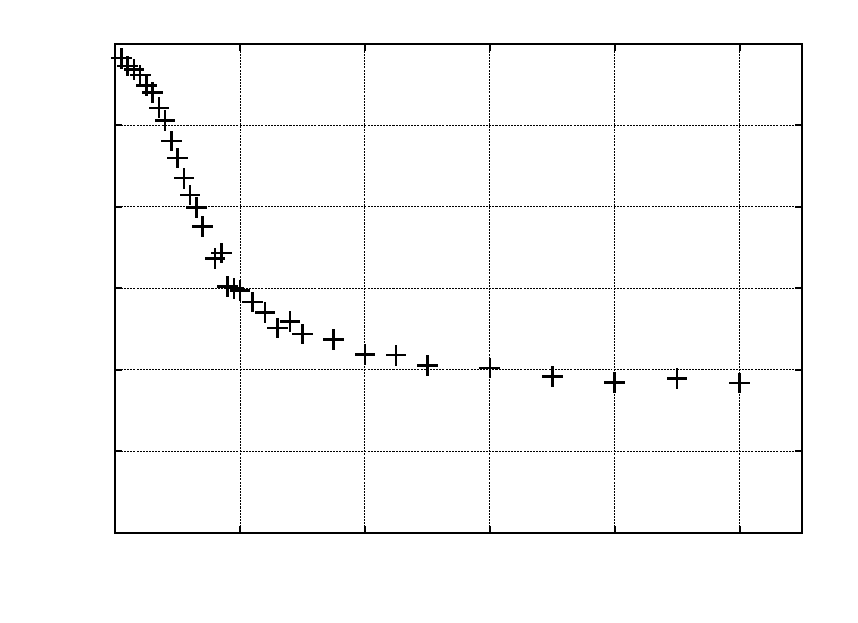
\includegraphics{RLCf}}%
    \gplfronttext
  \end{picture}%
\endgroup

\caption{Fázový posun proudu vůči napětí v RLC obvodu v závislosti na $C$}
\label{g:RLCf}
\end{graph}

\begin{graph}[htbp] 
\centering
% GNUPLOT: LaTeX picture with Postscript
\begingroup
  \makeatletter
  \providecommand\color[2][]{%
    \GenericError{(gnuplot) \space\space\space\@spaces}{%
      Package color not loaded in conjunction with
      terminal option `colourtext'%
    }{See the gnuplot documentation for explanation.%
    }{Either use 'blacktext' in gnuplot or load the package
      color.sty in LaTeX.}%
    \renewcommand\color[2][]{}%
  }%
  \providecommand\includegraphics[2][]{%
    \GenericError{(gnuplot) \space\space\space\@spaces}{%
      Package graphicx or graphics not loaded%
    }{See the gnuplot documentation for explanation.%
    }{The gnuplot epslatex terminal needs graphicx.sty or graphics.sty.}%
    \renewcommand\includegraphics[2][]{}%
  }%
  \providecommand\rotatebox[2]{#2}%
  \@ifundefined{ifGPcolor}{%
    \newif\ifGPcolor
    \GPcolorfalse
  }{}%
  \@ifundefined{ifGPblacktext}{%
    \newif\ifGPblacktext
    \GPblacktexttrue
  }{}%
  % define a \g@addto@macro without @ in the name:
  \let\gplgaddtomacro\g@addto@macro
  % define empty templates for all commands taking text:
  \gdef\gplbacktext{}%
  \gdef\gplfronttext{}%
  \makeatother
  \ifGPblacktext
    % no textcolor at all
    \def\colorrgb#1{}%
    \def\colorgray#1{}%
  \else
    % gray or color?
    \ifGPcolor
      \def\colorrgb#1{\color[rgb]{#1}}%
      \def\colorgray#1{\color[gray]{#1}}%
      \expandafter\def\csname LTw\endcsname{\color{white}}%
      \expandafter\def\csname LTb\endcsname{\color{black}}%
      \expandafter\def\csname LTa\endcsname{\color{black}}%
      \expandafter\def\csname LT0\endcsname{\color[rgb]{1,0,0}}%
      \expandafter\def\csname LT1\endcsname{\color[rgb]{0,1,0}}%
      \expandafter\def\csname LT2\endcsname{\color[rgb]{0,0,1}}%
      \expandafter\def\csname LT3\endcsname{\color[rgb]{1,0,1}}%
      \expandafter\def\csname LT4\endcsname{\color[rgb]{0,1,1}}%
      \expandafter\def\csname LT5\endcsname{\color[rgb]{1,1,0}}%
      \expandafter\def\csname LT6\endcsname{\color[rgb]{0,0,0}}%
      \expandafter\def\csname LT7\endcsname{\color[rgb]{1,0.3,0}}%
      \expandafter\def\csname LT8\endcsname{\color[rgb]{0.5,0.5,0.5}}%
    \else
      % gray
      \def\colorrgb#1{\color{black}}%
      \def\colorgray#1{\color[gray]{#1}}%
      \expandafter\def\csname LTw\endcsname{\color{white}}%
      \expandafter\def\csname LTb\endcsname{\color{black}}%
      \expandafter\def\csname LTa\endcsname{\color{black}}%
      \expandafter\def\csname LT0\endcsname{\color{black}}%
      \expandafter\def\csname LT1\endcsname{\color{black}}%
      \expandafter\def\csname LT2\endcsname{\color{black}}%
      \expandafter\def\csname LT3\endcsname{\color{black}}%
      \expandafter\def\csname LT4\endcsname{\color{black}}%
      \expandafter\def\csname LT5\endcsname{\color{black}}%
      \expandafter\def\csname LT6\endcsname{\color{black}}%
      \expandafter\def\csname LT7\endcsname{\color{black}}%
      \expandafter\def\csname LT8\endcsname{\color{black}}%
    \fi
  \fi
  \setlength{\unitlength}{0.0500bp}%
  \begin{picture}(7936.00,5668.00)%
    \gplgaddtomacro\gplbacktext{%
      \csname LTb\endcsname%
      \put(946,704){\makebox(0,0)[r]{\strut{} 0}}%
      \csname LTb\endcsname%
      \put(946,1226){\makebox(0,0)[r]{\strut{} 0.2}}%
      \csname LTb\endcsname%
      \put(946,1748){\makebox(0,0)[r]{\strut{} 0.4}}%
      \csname LTb\endcsname%
      \put(946,2270){\makebox(0,0)[r]{\strut{} 0.6}}%
      \csname LTb\endcsname%
      \put(946,2792){\makebox(0,0)[r]{\strut{} 0.8}}%
      \csname LTb\endcsname%
      \put(946,3315){\makebox(0,0)[r]{\strut{} 1}}%
      \csname LTb\endcsname%
      \put(946,3837){\makebox(0,0)[r]{\strut{} 1.2}}%
      \csname LTb\endcsname%
      \put(946,4359){\makebox(0,0)[r]{\strut{} 1.4}}%
      \csname LTb\endcsname%
      \put(946,4881){\makebox(0,0)[r]{\strut{} 1.6}}%
      \csname LTb\endcsname%
      \put(946,5403){\makebox(0,0)[r]{\strut{} 1.8}}%
      \csname LTb\endcsname%
      \put(1078,484){\makebox(0,0){\strut{} 0}}%
      \csname LTb\endcsname%
      \put(2253,484){\makebox(0,0){\strut{} 2}}%
      \csname LTb\endcsname%
      \put(3427,484){\makebox(0,0){\strut{} 4}}%
      \csname LTb\endcsname%
      \put(4602,484){\makebox(0,0){\strut{} 6}}%
      \csname LTb\endcsname%
      \put(5777,484){\makebox(0,0){\strut{} 8}}%
      \csname LTb\endcsname%
      \put(6952,484){\makebox(0,0){\strut{} 10}}%
      \put(176,3053){\rotatebox{-270}{\makebox(0,0){\strut{}$P$ (\si{\watt})}}}%
      \put(4308,154){\makebox(0,0){\strut{}$C$ (\si{\micro\farad})}}%
    }%
    \gplgaddtomacro\gplfronttext{%
    }%
    \gplbacktext
    \put(0,0){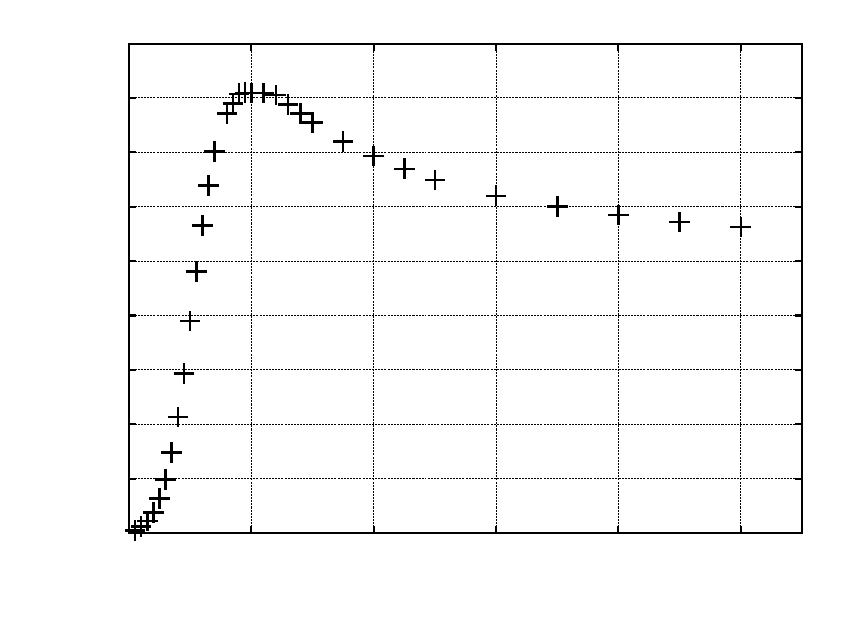
\includegraphics{RLCP}}%
    \gplfronttext
  \end{picture}%
\endgroup

\caption{Výkon RLC obvodu v závislosti na $C$}
\label{g:RLCP}
\end{graph}


Sériový RC obvod jsme připojili k osciloskopu.
Při nulové kapacitě bylo napětí na kondenzátoru a na rezistoru ve fázi a mělo stejnou amplitudu. Když jsme poté kapacitu zvyšovali, napětí na kondenzátoru se snižuje a posouvá vůči napětí na rezistoru.